\documentclass[11pt]{article}
\usepackage[utf8]{inputenc}
\usepackage[T1]{fontenc}
\usepackage{minted}
\usepackage{graphicx}
\usepackage{hyperref}

\author{Student: Sean Wang, szw87 \\ Professor: Mohit Tiwari, Antonio Espinoza \\ Department of Electrical \& Computer Engineering \\ The University of Texas at Austin}
\date{\today}
\title{EE379K Enterprise Network Security Lab 1 Report}
\hypersetup{
 pdfauthor={Student: Sean Wang, szw87 \\ Professor: Mohit Tiwari, Antonio Espinoza \\ Department of Electrical \& Computer Engineering \\ The University of Texas at Austin},
 pdftitle={EE379K Enterprise Network Security Lab 1 Report},
 pdfkeywords={},
 pdfsubject={},
 pdfcreator={},
 pdflang={English}}

\begin{document}

\maketitle
\section*{Part 1 - Networking and Denial of Service}
\subsection*{Step 1 - Client and Server in C}
For step 1, the client and server in C were implemented to closely match the Python versions.
For simplicity, the client sends the same hard coded message each time, similar to the Python
client. The C client and server were tested with the Python client and server to ensure
cross-functionality and that the client implementation in both languages worked almost
identically. The only difference between the C client and Python client was the output of the
Python client showing
\begin{verbatim}
  From Server: b'INPUT LOWERCASE SENTENCE:'
\end{verbatim}
and the C client showing
\begin{verbatim}{bash}
  From Server: INPUT LOWERCASE SENTENCE:
\end{verbatim}
To build the server, compile it with:
\begin{minted}{bash}
  $ gcc -o server server.c
\end{minted}
Similarly for the client, compile it with:
\begin{minted}{bash}
  $ gcc -o client client.c
\end{minted}
To run them, simply execute either:
\begin{minted}{bash}
  $ ./server
  $ ./client
\end{minted}
\subsection*{Step 2 - DOS Attack}
For step 2, the DOS attack was implemented using a command line tool called \verb|hping3| using
the options
\begin{minted}{bash}
  $ sudo hping3
      --count 15000 \           # number of packets
      --destport 12000 \        # destination port
      --rand-source \           # randomize source IP
      --flood \                 # send as fast as possible
      --syn \                   # send SYN packets
      127.0.0.2                 # destination IP
\end{minted}
These flags specify to stop sending packets to \verb|127.0.0.2:12000| after sending/receiving 15000
SYN packets, using randomized IP addresses to disguise the actual source and prevent the
server's SYN-ACK packets from reaching the actual source. Additionally, the \verb|--flood|
option just says to send packets as fast as possible.\\
As a result, the server receives many requests for establishing a connection, but because the
SYN-ACK sent from the server never reaches the actual sender of the initial SYN packet, the
3-way handshake is never completed and the server is left waiting on a response from what it
sees as many clients. This can be seen in Figure~\ref{fig:handshake}, with some packet details
cut out to ensure legibility.
\begin{figure}[htbp]
  \centering
  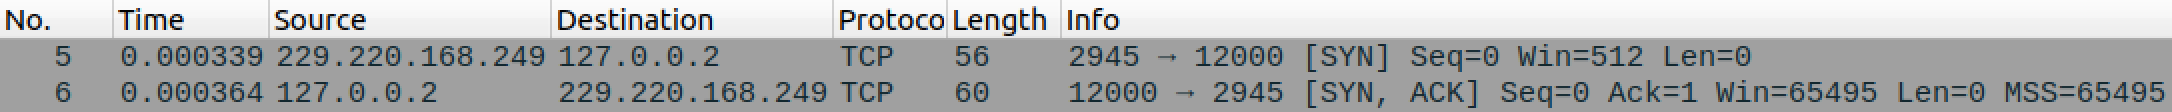
\includegraphics[width=1\linewidth]{./incomplete_handshake.png}
  \caption{\label{fig:handshake}
  An incomplete three-way handshake}
\end{figure}
\\
Since the server is now swamped with connection requests, the real client (at IP \verb|127.0.0.1|)
cannot have its connection request processed by the server and times out, as shown in
Figure~\ref{fig:timeout}, also with some packet details cut out to ensure legibility.
\begin{figure}[htbp]
  \centering
  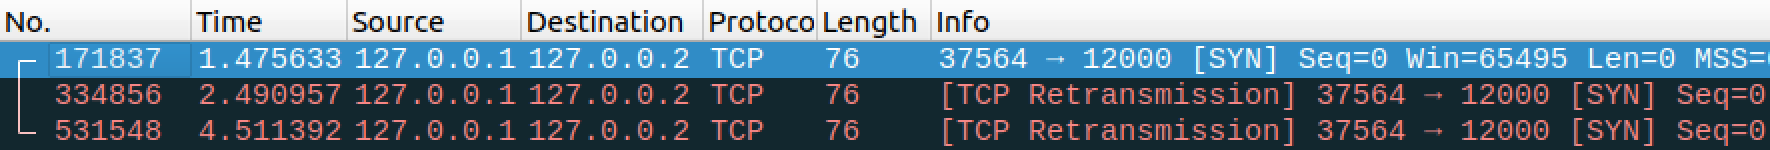
\includegraphics[width=1\linewidth]{./client_timeout.png}
  \caption{\label{fig:timeout}
  Client's sent SYN packet and client timeout}
\end{figure}
\\
The rest of the tcpdump record of the DOS attack is in \verb|output.pcap| and shows the flood
of SYN packets sent to the server at IP \verb|127.0.0.2:12000|.
\section*{Part 2 - zmap scan}
For this part, a zmap scan was run for about 2 hours and 47 minutes (10000 seconds) with the
following options:
\begin{minted}{bash}
  $ sudo zmap \
      --blacklist-file=blacklist.conf \ # subnets to exclude
      --target-port=80 \                # port number to scan
      --output-file=zmap_result.txt \   # output file
      --max-runtime=10000               # max runtime (seconds)
\end{minted}
\section*{Part 3 - Internet Traffic On Different Connections}
For this part, a script (\verb|auto_collect.sh|) was used to automate accessing 10 different
websites 10 times each and recording network traffic with \verb|tcpdump|. This script was run
once per connection type (VPN, TOR, Firefox). Afterwards, another script (\verb|auto_summarize.sh|)
was used to automate summarizing the resulting \verb|.pcap| files for packets sent per access
and the average packet size per access. The collected data regarding the average number of packets
is summarized in Figure~\ref{fig:avg_packets} and the data regarding the average size of packets
is summarized in Figure~\ref{fig:avg_size}.\\
Using just a regular browser to access the websites, a passive device on the network can see
all kinds of information, including which websites were visited and the sizes of the packets. With a
VPN, \verb|tcpdump| captured information showing the client sending packets to the VPN server and
vice versa. However, information regarding packet source and destination were still visible. Finally,
using TOR, the captured network traffic showed mostly packets being sent to and from \verb|127.0.0.1|
and not the IP of, say, \verb|wikipedia.org|. As a result, it was much harder to tell exactly what
websites were visited just by looking at network traffic in Wireshark.\\
Although difficult, it is possible to determine which of the 10 websites was visited simply based on
connection statistics. For example, in Figure~\ref{fig:avg_size}, UC Berkeley's website has, on average,
larger packet sizes than most of the other websites, so given only these basic connection statistics,
guessing UC Berkeley's website as the site visited due to large packet sizes is not unreasonable.
Additionally, connection statistics that show a consistent rate packets sent and a consistent packet
size would most likely imply that a video or stream was being watched.\\
Some other observations of note were in regards to the number of packets sent per connection. The 
average number of packets sent each iteration of visiting the same website generally decreased as the
website was visited more. Also, since the websites were visited in a consistent order (from left to 
right on Figure~\ref{fig:avg_packets} and Figure~\ref{fig:avg_size}), there seemed to be a consistent
trend of decreasing average number of packets per connection. 
\begin{figure}[p]
  \centering
  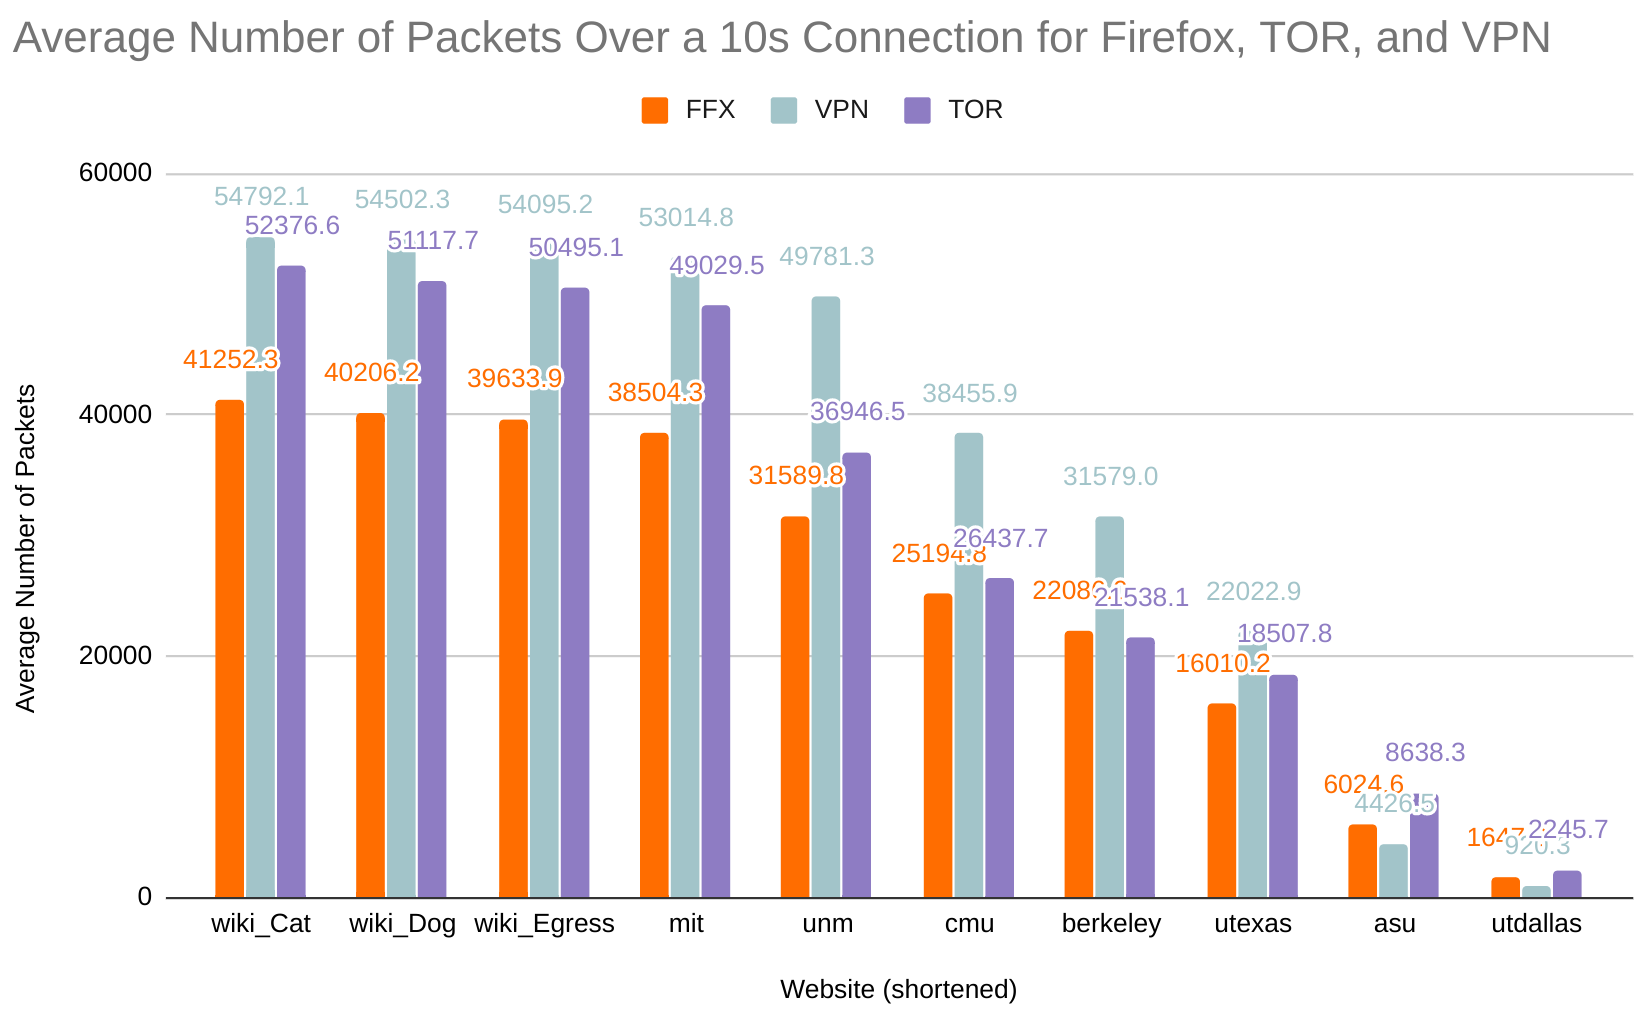
\includegraphics[width=1\linewidth]{./average_packets.png}
  \caption{\label{fig:avg_packets}
  The average number of packets sent over a 10 second connection for 10 different websites on 3 different connections}
\end{figure}
\begin{figure}[p]
  \centering
  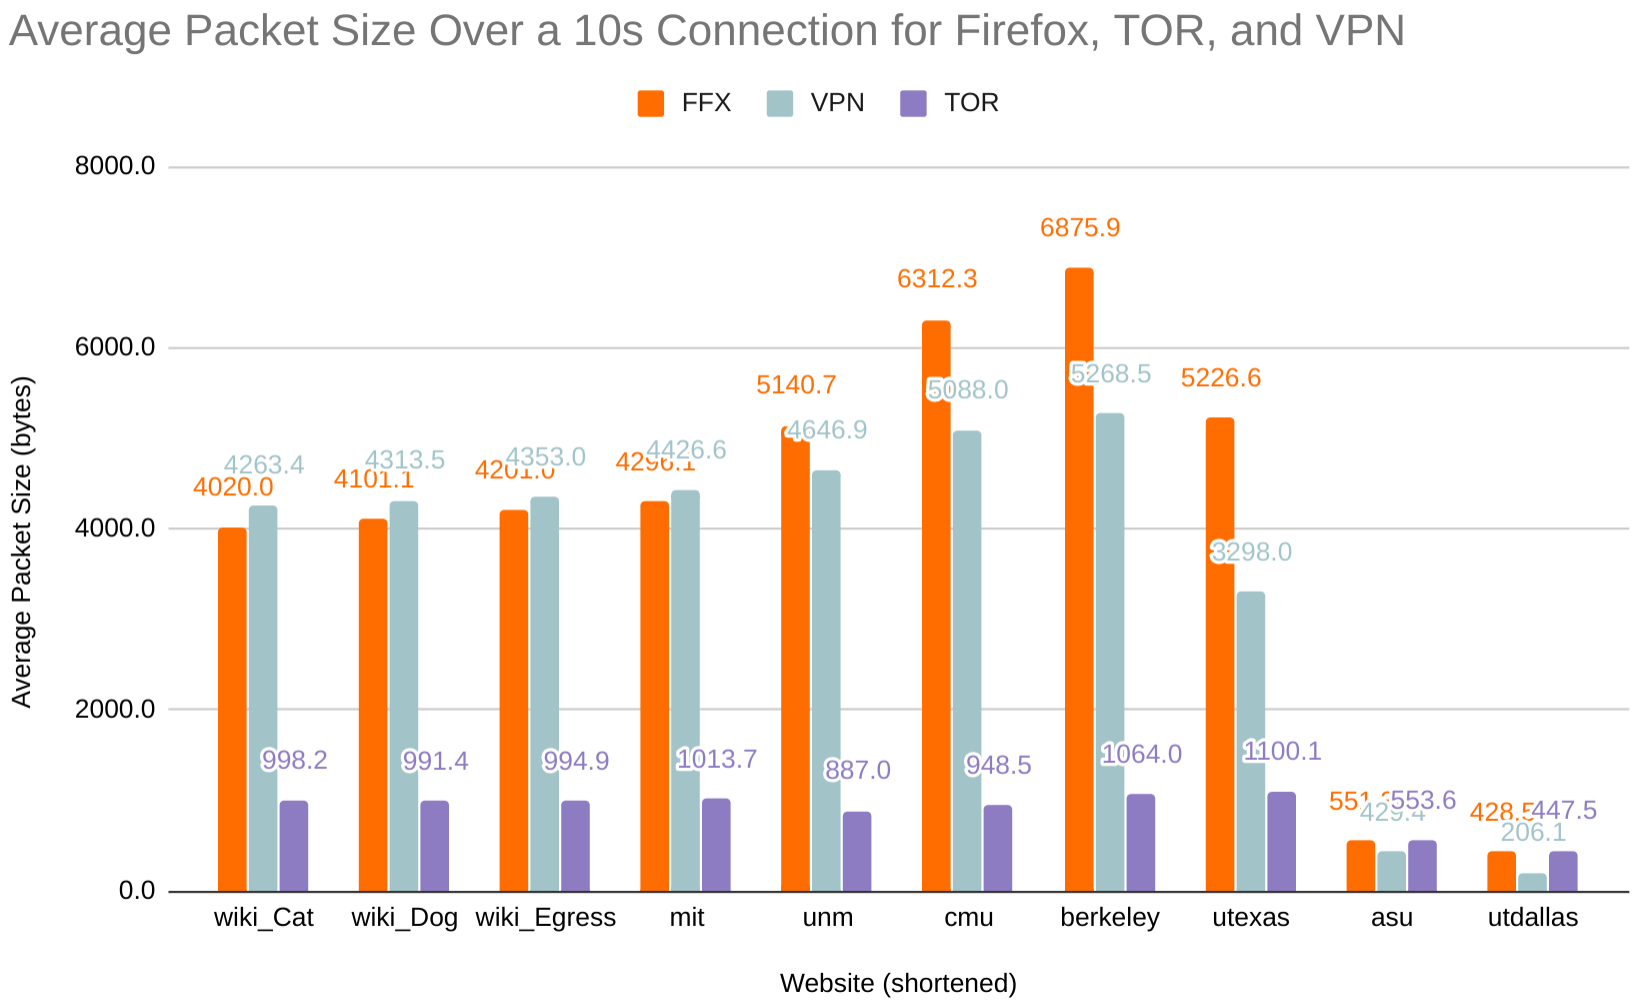
\includegraphics[width=1\linewidth]{./average_size.png}
  \caption{\label{fig:avg_size}
  The average size of packets sent over a 10 second connection for 10 different websites on 3 different connections}
\end{figure}
\section*{Part 4:}

% \label{part1:step-1}
% Nam dui ligula, fringilla a, euismod sodales, sollicitudin vel, wisi. Morbi
% auctor lorem non justo. Nam lacus libero, pretium at, lobortis vitae, ultricies
% et, tellus. Donec aliquet, tortor sed accumsan bibendum, erat ligula aliquet
% magna, vitae ornare odio metus a mi. Morbi ac orci et nisl hendrerit mollis.
% Suspendisse ut massa. Cras nec ante. Pellentesque a nulla. Cum sociis natoque
% penatibus et magnis dis parturient montes, nascetur ridiculus mus. Aliquam
% tincidunt urna. Nulla ullamcorper vestibulum turpis. Pellentesque cursus luctus
% mauris.

\end{document}
